%!TEX root = ../../thesis.tex


\section{Results of spectral differential analysis}
\label{subsec:differential_results}

\begin{figure}
    \centering
    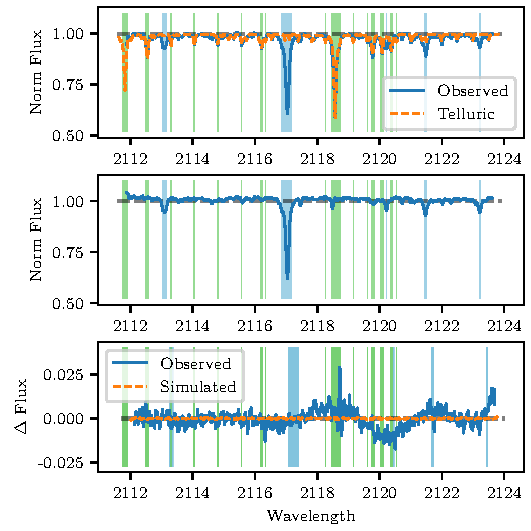
\includegraphics[width=0.8\hsize]{figures/direct-recovery/differential.pdf}\\
    \caption[Example of the spectral differential technique.]{Top: A reduced {CRIRES} observation of {HD\,30501} (blue) for detector 1 between 2112--2124\nm{} along with the {TAPAS} telluric absorption model ({orange} dashed) used for the wavelength calibration and telluric correction.
        Middle: The telluric corrected spectra.
        Bottom: ({blue}) Differential spectra for {HD\,30501} between observations 1 and 3.
        ({orange} dashed) Simulated ``perfect'' differential using {PHOENIX-ACES} spectra with parameters \Teff{}=2500\K{}, \Logg{}=5.0, and \feh{}=0.0, with the same \(\Delta {RV}\) as the observations.
        The shaded regions indicate where the telluric {green} and host star {blue} spectra are \(> 4\%\) deep.}
    \label{fig:spectral_example}
\end{figure}


The spectral differential procedure outlined above was applied to the wavelength-calibrated, telluric- and barycenter- corrected {CRIRES} observations.
The spectra were first Doppler shifted to the rest frame velocity of the system by applying a shift of \(-\gamma\).
Each spectra is then shifted by its $-{RV}_{1}$ so that the host lines are at rest.
Finally one spectrum is subtracted from the other as described above.

Although this is attempted on all targets only the most favourable case, {HD\,30501}, is shown in \cref{fig:spectral_example}.
It is favourable because it is the second largest companion in the sample at 90~\Mjup{} but also has the second largest {RV} separation between observations.
The top panel shows the reduced CRIRES spectrum of {HD 30501} from detector 1 without telluric correction.
The telluric model is also shown in the top panel.
The middle panel shows the CRIRES spectra corrected with the telluric model.
The differential spectra recovered for {HD\,30501} is shown at the bottom panel of \cref{fig:spectral_example}.
The shaded regions indicate where the telluric {green} and host star {blue} spectra are \(> 4\%\) deep.
This indicates that the features of the differential spectrum near these shaded regions are likely due to imperfect telluric correction and host cancellation.

The mutual cancellation of the stellar host seems to work well for the \(\sim40\%\) deep line near 2117\nm{}, with the line being completely removed, but it does not do so well for the smaller \(\sim10\%\) deep line around 2121.5\nm{}.
The residual for the large \(\sim40\%\) deep telluric line near 2118.5\nm{} is still quite prominent.
Around 2120\nm{} there is wide negative residual around three neighbouring telluric lines, \(\sim10\%\) deep.
One possible explanation for this is that the continuum normalization near 2120\nm{} was influenced by this grouping of lines.

To understand the observed differential signal simulations were performed of a differential spectrum of {HD\,30501} using a synthetic {PHOENIX-ACES} spectra with parameters \Teff{}=2500\K{}, \Logg{}=5.0, and \feh{}=0.0, with the {RV} offset estimated from the observation times.
These parameters represent an estimated companion \Teff{} with the metallicity and \Logg{} similar to the host (closest grid model).
The model spectra were convolved to \(\R=50\,000\), continuum normalized and scaled by the estimated flux ratio of the companion.
In this simulation a synthetic host or telluric spectra is not included and as such simulates the differential result of a ``perfect'' host cancellation with no telluric contamination present.
This is the ideal-case scenario, and it is stressed that it is impossible to simulate the effect of improper telluric correction in a meaningful way.
When comparing the simulated and observed differential in the bottom panel of \cref{fig:spectral_example}, there is a striking amplitude difference.
The orange-dashed line of the simulated differential spectrum amplitude is of a much smaller scale than the observed differential.
This simulation demonstrates that the amplitude of the differential signal of {HD 30501} expected is much smaller than the residuals created by the differential technique applied to these observations.

The amplitude of the differential signal is lower than expected due to the very low \(\Delta {RV}\) between the observation pairs.
The maximum \(\Delta {RV}\) between observational pairs, for the targets investigated in this work, are provided in \cref{tab:estimated_rv}.
In the best target in this sample, {HD\,30501}, the \(\Delta {RV}_2\) of the companion between observations is 1.41\kmps{}.
For comparison, a single Gaussian absorption line, to be shifted by \(\Delta\lambda = {\fwhm}\) would need a \(\Delta {RV}\) of \(v_{\fwhm} = c/\R \approxeq\sim6\)\kmps{}.
Since the \(\Delta {RV}_2\) are shifted by a significant smaller value than the line {\fwhm}, the spectral lines of the companion also mutually cancel themselves, diminishing the amplitude of the differential signal significantly.
As the companion spectra are already faint (with a flux ratio at the percent level) the differential signal is not detectable in these observations at the achieved noise level.

When the \(\Delta {RV}\) of the companion is smaller than the {\fwhm} of a line there is a mutual subtraction of the companion spectra, diminishing the detected amplitude of the differential signal, and removing the ability to detect the companions using this method.
THe observations need to be spaced further apart in time/phase to achieve a larger \(\Delta {RV}_2\) separation and increase the amplitude of the differential.
Once there is a separation there will be complex interactions between neighbouring lines that need to be accounted for.


